\documentclass[conference]{IEEEtran}
\IEEEoverridecommandlockouts
% The preceding line is only needed to identify funding in the first footnote. If that is unneeded, please comment it out.
\usepackage{cite}
\usepackage{amsmath,amssymb,amsfonts}
\usepackage{algorithmic}
\usepackage{graphicx}
\usepackage{textcomp}
\usepackage{subfigure}
\usepackage{caption}
\usepackage{graphicx} %use graph format
\usepackage{epstopdf}

\def\BibTeX{{\rm B\kern-.05em{\sc i\kern-.025em b}\kern-.08em
    T\kern-.1667em\lower.7ex\hbox{E}\kern-.125emX}}

\newcommand{\tabincell}[2]{\begin{tabular}{@{}#1@{}}#2\end{tabular}}
    
\begin{document}

\title{A Hybrid Model based on Multi-Dimensional Features for Insider Threat Detection\\
\thanks{Identify applicable funding agency here. If none, delete this.}
}

\author{\IEEEauthorblockN{ Bin Lv \textsuperscript{1,2},
Dan Wang\textsuperscript{1,2},
Yan Wang\textsuperscript{1*},
Qiujian Lv\textsuperscript{1,2},
Dan Lu\textsuperscript{1,2}
}
\IEEEauthorblockA{\textsuperscript 1Institute of Information Engineering, Chinese Academy of Sciences, Beijing 100093, China \\
\textsuperscript2School of Cyber Security, University of Chinese Academy of Sciences, Beijing 100049, China\\
Email:\{lvbin, wangdan3, wangyan, lvqiujian, ludan\}@iie.ac.cn\\
\textsuperscript *Corresponding author}
\iffalse
\and
\IEEEauthorblockN{2\textsuperscript{nd} Given Name Surname}
\IEEEauthorblockA{\textit{dept. name of organization (of Aff.)} \\
\textit{name of organization (of Aff.)}\\
City, Country \\
email address}
\fi
}

\maketitle

\begin{abstract}
Insider threats have shown their power by hugely affecting national security, financial stability, and the privacy of many thousands of people.
A number of techniques have been proposed to detect insider threats either by comparing behaviors among different individuals or by comparing the behaviors across different time periods of the same individual. However, due to the fact that the behaviors of insider threats are always complex and diverse, both of them always fail to identify certain kinds of inside threats.
This paper focuses on proposing a hybrid model to detect insider threats based on multi-dimensional features.
First, based on the isolation Forest algorithm,  
an Across-Domain Anomaly Detection (ADAD) model is proposed to identify anomalous behaviors that deviate from the behaviors of their peers by using multi-source information. Second, we propose an Across-Time Anomaly Detection (ATAD) model to measure the degree of unusual changes of a user's behavior by implementing an improvement model based on Markov. Finally, our proposed hybrid model presents a fusion
method to integrate the evidence from the above two models. With the data lasting 17 months, we evaluate our proposed models comprehensively. The results demonstrate the robust performance of the ADAD and ATAD models and the hybrid model is demonstrated to outperform the two separate models obviously.


\end{abstract}

\begin{IEEEkeywords}
insider threat detection, information fusion, hybrid model, Isolation Forest, Markov Model
\end{IEEEkeywords}

\section{Introduction}

Insider threats are threats with malicious intent directed towards organizations by people internal to the organization \cite{b1}.
These include physical sabotage activities, theft of confidential data and business secrets, and fraud. Financial loss and reputation damage caused by this ``known unknow'' cybersecurity threat far outweighs that caused by external attacks. One of the most recent articles from CSO magazine \cite{b2} compared the cost between external and internal attacks and noted that while it takes about 50 days to fix a data breach caused by an internal attack, it only takes 2 to 5 days in the case of external attacks. Nowadays, researchers have proposed different models to prevent or detect the presence of attacks.

\begin{figure*}[htb]
\centerline{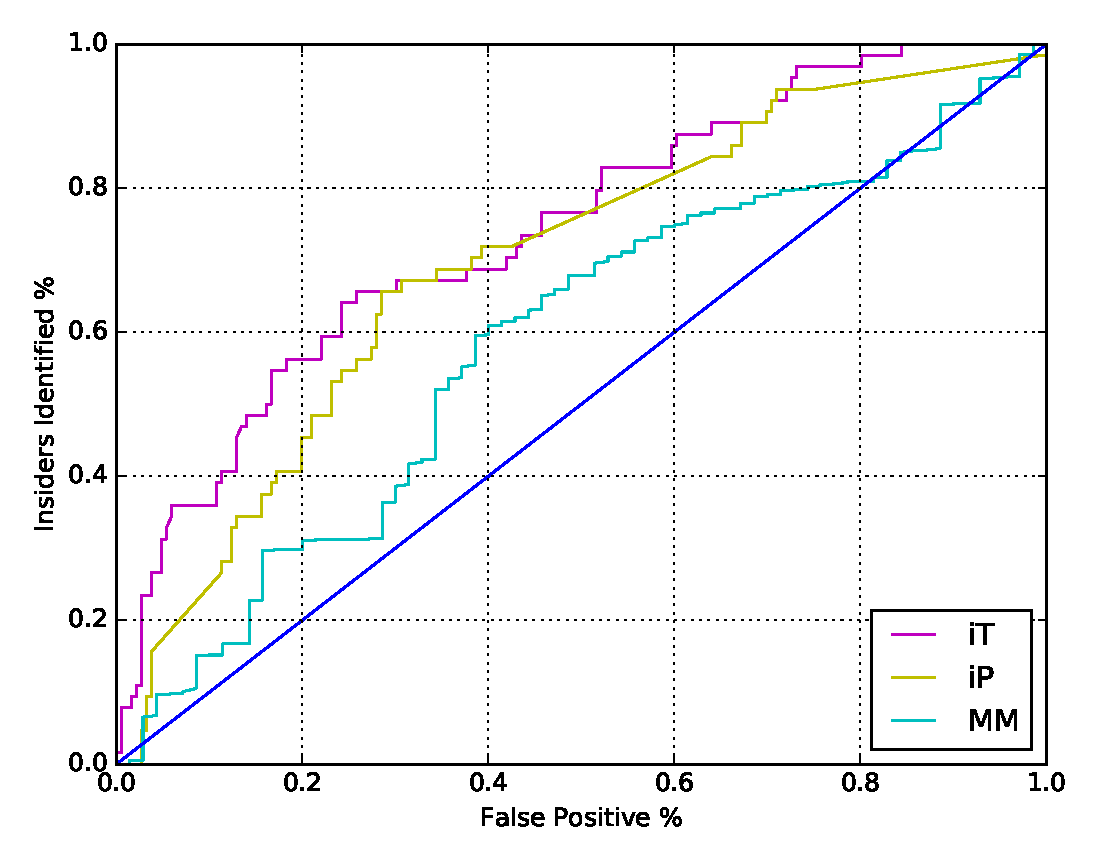
\includegraphics[width = 0.7\textwidth]{figure/figure1.eps}}
\caption{Example of insider threat.}
\label{fig}
\end{figure*}

Existing literature focuses on two types of insider threat detection 
models: data-driven detection models \cite{b3},\cite{b4} and behavior driven detection models \cite{b5},\cite{b6}: 

\noindent \emph{1)} The first model aims to find a normal portrait in all users data in order to detect insider threat that deviates from this normal portrait by comparing with their peers \cite{b7}. Fig. 1 shows an example of insider threats which can be detected by this kind of model \cite{b7}. After getting off work, the general behavior is going home to have a rest. By contrast, few of users secretly deal with the company's confidential documents in the workplace when others are sunk in sleep at midnight, and are more likely to be an insider threat. However, merely comparing the behaviors among peers,  this kind of models fails to detect a malicious insider who tries to behave like a normal user to cover up his evil.

\noindent \emph{2)} The second model regards the abnormal changes in the behavior as the basis for insider threat detection by comparing behaviors of themselves in different time periods.
Fig. 1 also shows an example to depict a malicious insiders detection based on the behavior-driven method \cite{b8}. Over a long period in the past, the regular behavior of the user was to click on the browser after booting, view the email, and then reply. But one day, he acted abnormally: he connected the mobile device after booting, and had a series of operations on the file-copy to steal the company's confidential documents. These abnormal behaviors don't match his usual styles of doing things. It is worth to note that although the malicious insider may try to behave like a normal user, the threat can also be detected based on the deviation from his regular behavior routines.
However, the model is unable to recognize situations where a user systematically attacks an
organization over a long-term period \cite{b3}. 

Thus, Insider threat surveys \cite{b9} suggest the problem of insider threat detection cannot be defined only as a data or behavior driven problem. Therefore, it is necessary to model the problem as data and behavior driven problems, based on which an effective model needs to be proposed.

Hence, based on multidimensional features, this paper proposes a hybrid model that combines a data-driven model with a behavior driven model to detect insider threat in a more robust and accurate manner.
First, the multi-dimensional features extracted from data collected from an enterprise network is formatted and fed separately into the two separate models. Second, each model generates an abnormal score to represent the degree of users' unusual behaviors. Finally, the abnormal scores of two models are fused to be the final abnormal score of each user, and a user is identified to be an insider threat if the anomaly score exceeds the threshold. 
After a wide range experiments, it is 
verified that the hybrid model can detect insider threats in a more robust and accurate manner.
Overall, the contributions of this paper can be summarized as follows:


\begin{enumerate}
\item 
We apply the isolation Forest to detect behavioral inconsistencies among the behaviors of users. In this model, we extract temporal features from multi-source data and combine them comprehensively when constructing the user's portrait.

\item We propose an improved model based on Markov to identify users' unusual changes. The proposed model considers all historical behaviors of users as the contextual information. As compared with the existing detection methods of Markov model \cite{b7}, our proposed approach show higher efficiency.


\item We propose a hybrid model based on multi-dimensional features for insider threat detection. The model is able to determine malicious insiders that not only act inconsistent with their peers but also have unusual changes compared with their historic behaviors. 
Through extensive experiments, we obtain the accuracy of 95\% through the proposed model, which is of great significance in industry and scientific research.
 


\end{enumerate}

The remainder of this article is structured as follows. 
Section II presents the related work.
Then, section III details our approach. Next, in section V, 
we detail our implementation of the models and analyze the results of experiments. 
Finally, we conclude in section VI, also presenting limitation of our work.




\section{Related work}
%在增加一部分related work:hybrid model 或者多特征融合
The topic of insider threat has recently received much attention in the literature. Researchers have proposed different models aimed at preventing or detecting the presence of attacks  \cite{b11},\cite{b12}. To elicit the state of art, the work
presented here is focused on the approaches of detecting insider threat based on data-driven methods and behavior-driven methods, respectively.

With regard to the data-driven methods, Mathew et al. \cite{b13} detected inside threat on account of user access patterns, Eberle et al. \cite{b14} used social graphs to detect the abnormal. More recently, Eldardiry et al. \cite{b15} have also proposed a system for managing insider attacks and compared user’s behavior based on peer baselines.
Michael Goldsmith applied a layered architecture by fusing across multiple levels information to detect anomalies from heterogeneous data \cite{b16}. Hoda et al. \cite{b13} detected peer groups of users and modeled user behavior with respect to these peer groups. Subsequently, they detected insider activity by identifying users who deviated from their peers. 
There have also been various other approaches based on data-driven to detect abnormal \cite{b10},\cite{b8}. 
However, they did not factor in the changes of user behaviors over time. We note that while a common activity is not suspicious, a rare change of the order common activity can be. 

There are several literatures based on behavior-driven models \cite{b7},\cite{b11},\cite{b12}. 
Tabish Rashid \cite{b17} took the change of the user's behavior over time to detect the anomaly and achieved some results. M. Bishop \cite{b11} examined the application of process modeling
and subsequent analyses to the insider problem. 
However, these behavior-driven models just work out based on unusual changes of user behaviors, and they will miss recognizing situations where a user systematically attacks an organization over an extended time-framework.



\section{Overview of proposed approach}
To detect insider threat that deviates from the portraits of normal users as well as who tries to behave like a normal user to cover up his evil,
we propose a hybrid model based on multi-dimensional features for insider threat detection. The structure of our proposed model is illustrated in Fig. 2. The hybrid model includes two components, one is named ``Across-Domain Anomaly Detection (ADAD)'', and the other is ``Across-Time Anomaly Detection (ATAD)''. We get anomaly scores from the two components, then fuse them as the basis for insider threat detection.  The multi-source information contains activities such as logging on/off, sending and receiving emails, accessing external devices or files, and
accessing web sites. We refer to different categories of data as “domains”, e.g., “logon domain” and “email domain”. The dataset used in this paper is described in the following section. 


\begin{figure}[htb]
\centerline{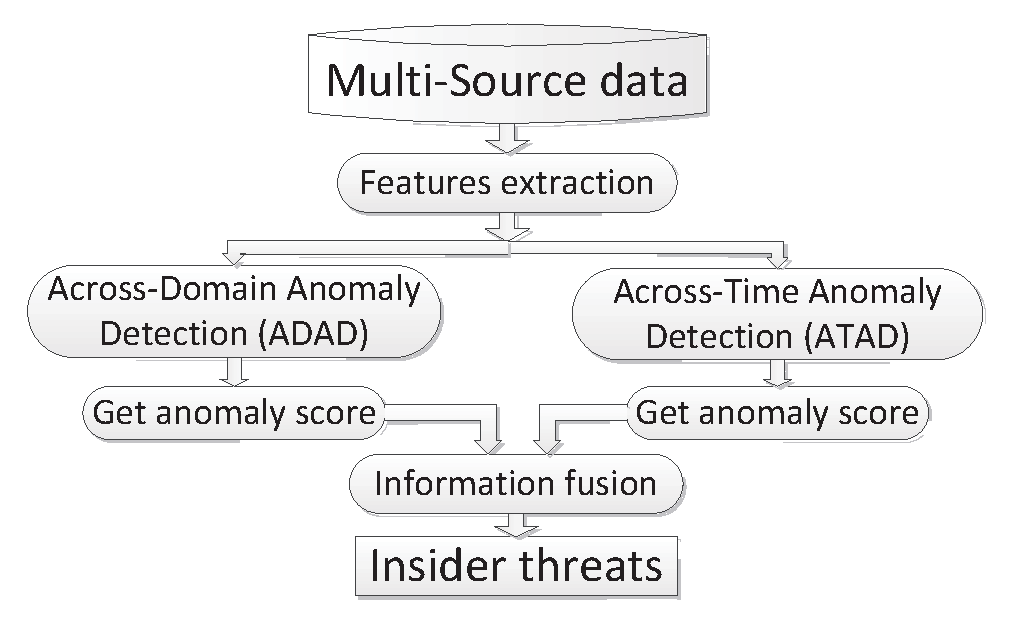
\includegraphics[width = 0.35\textwidth]{figure/figure2.eps}}
\caption{Anomaly detection framework.}
\label{fig}
\end{figure}

\subsection{The Data Set}

Due to the lack of availability of proper insider threat datasets, we have utilized the insider threat dataset published by CERT Carnegie Mellon University for this research \cite{b17}. The dataset ``R4.2.tar.bz'' lasting 17 months has been used for this analysis. This dataset consists of six broad types of data records (HTTP, logon, device, file, email and psychometric) of 1000 employees over a 17 months period. All HTTP records contain user, PC, URL and web page content with time stamps. “Logon.csv” consists of user logon/logoff activities with the corresponding PC with timestamps. The data file “device.csv” indicates insert/remove actions with the relevant user, PC, and timestamp. Details of file copies are stored in “file.csv” file with date, user, PC, filename, and content. We should note that the Dataset contains the ground truth for each user (when they are acting maliciously or not), which allows us to monitor the success or failure of our experiment.

\section{KEY METHODOLOGIES}
In this section, we describe our Across-Domain Anomaly Detection (ADAD) model in detail at first. We then detail the Across-Time Anomaly Detection (ATAD) model. Finally, we introduce the fusion method to combine ADAD and ATAD.

\subsection{Approach 1:Across-Domain Anomaly Detection (ADAD)}\label{AA}
This framework will utilize multi-domain information inputs, such as logon records and operation on file, to identify abnormal users, who behave differently from their peers. We first extract temporal features from multi-domain data, upon which insider threats are detected.

\iffalse
Figure 3 reports the structure of the approach.


\begin{figure}[htb]
\centerline{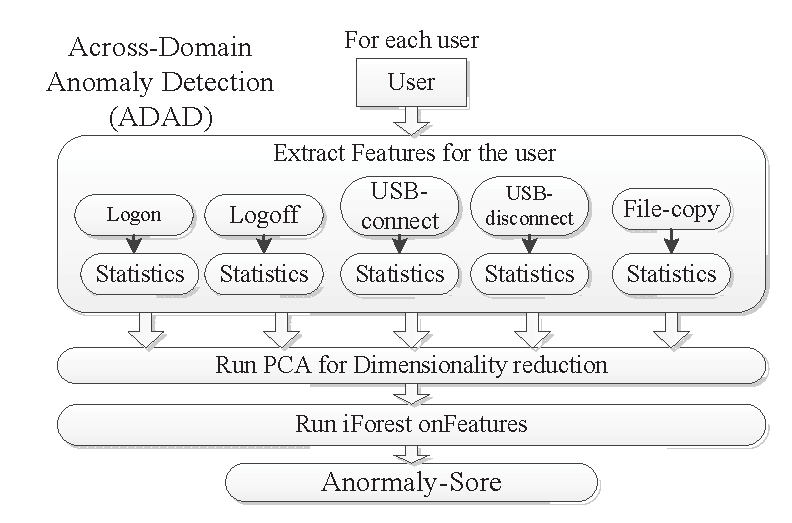
\includegraphics[width = 0.35\textwidth]{figure/figure3.eps}}
\caption{An overview of the Across-Domain Anomaly Detection (ADAD).}
\label{fig}
\end{figure}
\fi
\subsubsection{Feature Extraction}


\textbf{Logon/Logoff Behaviors.} 
As most disgruntled insiders tend to
commit malicious logon or logoff activities after hours,  these behaviors are applied to identify malicious insiders.

%width=2.8in


\begin{figure*}[!t]
\centering
\subfigure[Logon behavior]{
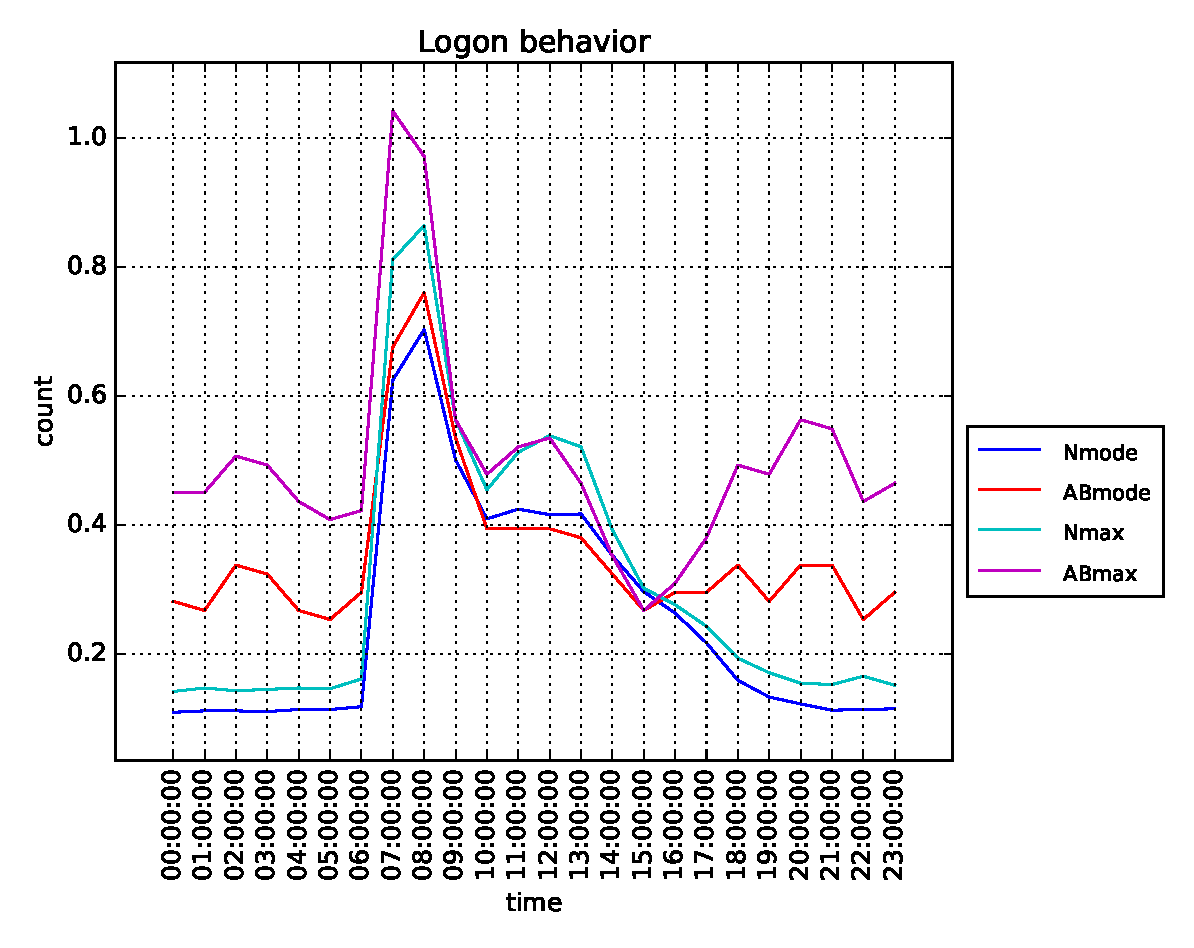
\includegraphics[width=0.18\textwidth]{figure/figure41.eps}
} 
\subfigure[Logoff behavior]
{
 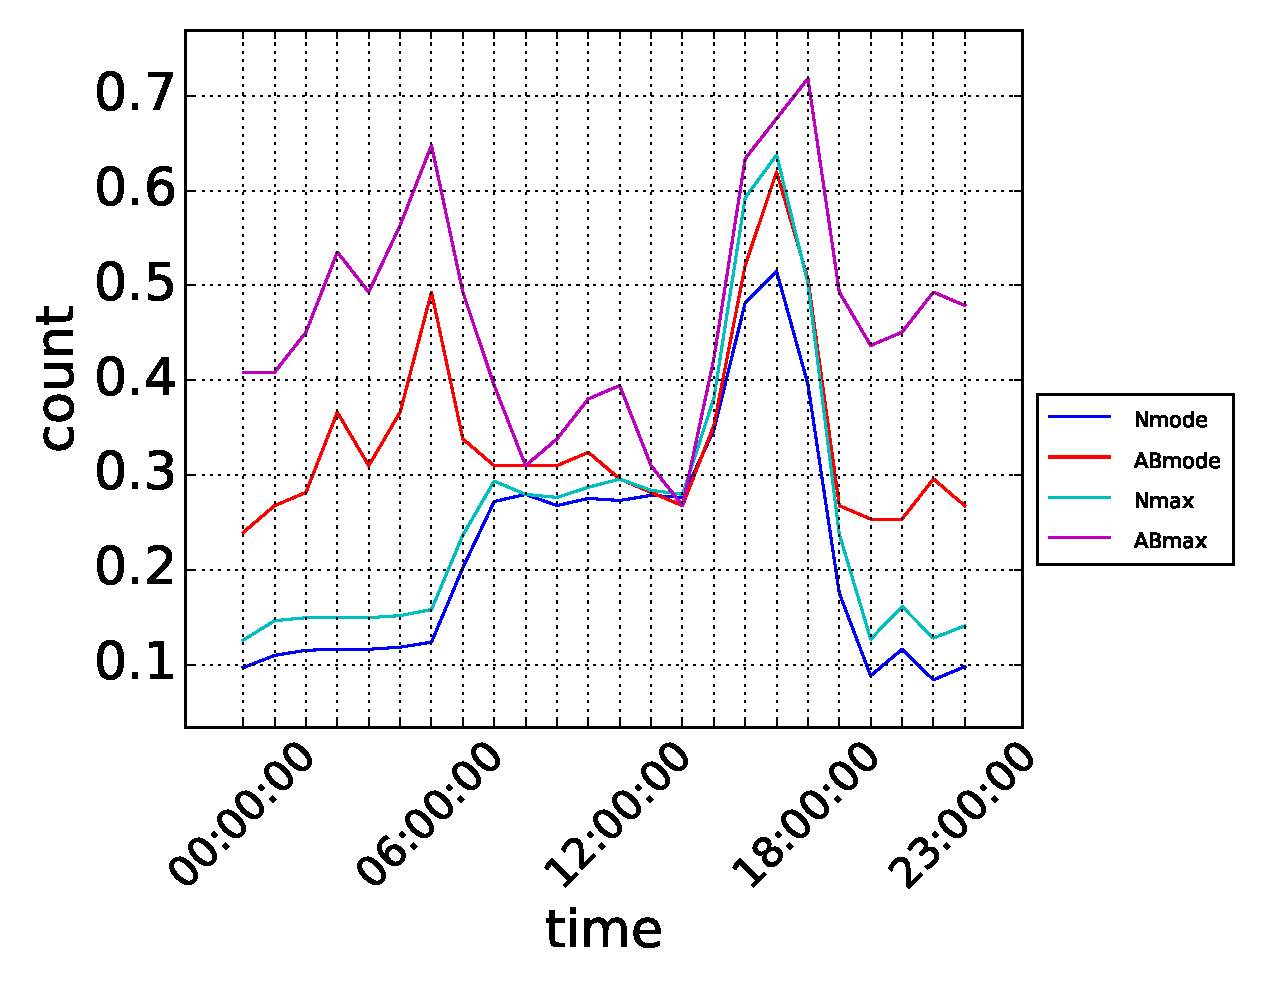
\includegraphics[width=0.18\textwidth]{figure/figure42.eps}
}
%\caption{ Users’ logon and logoff behavior }
\subfigure[USB connect]{
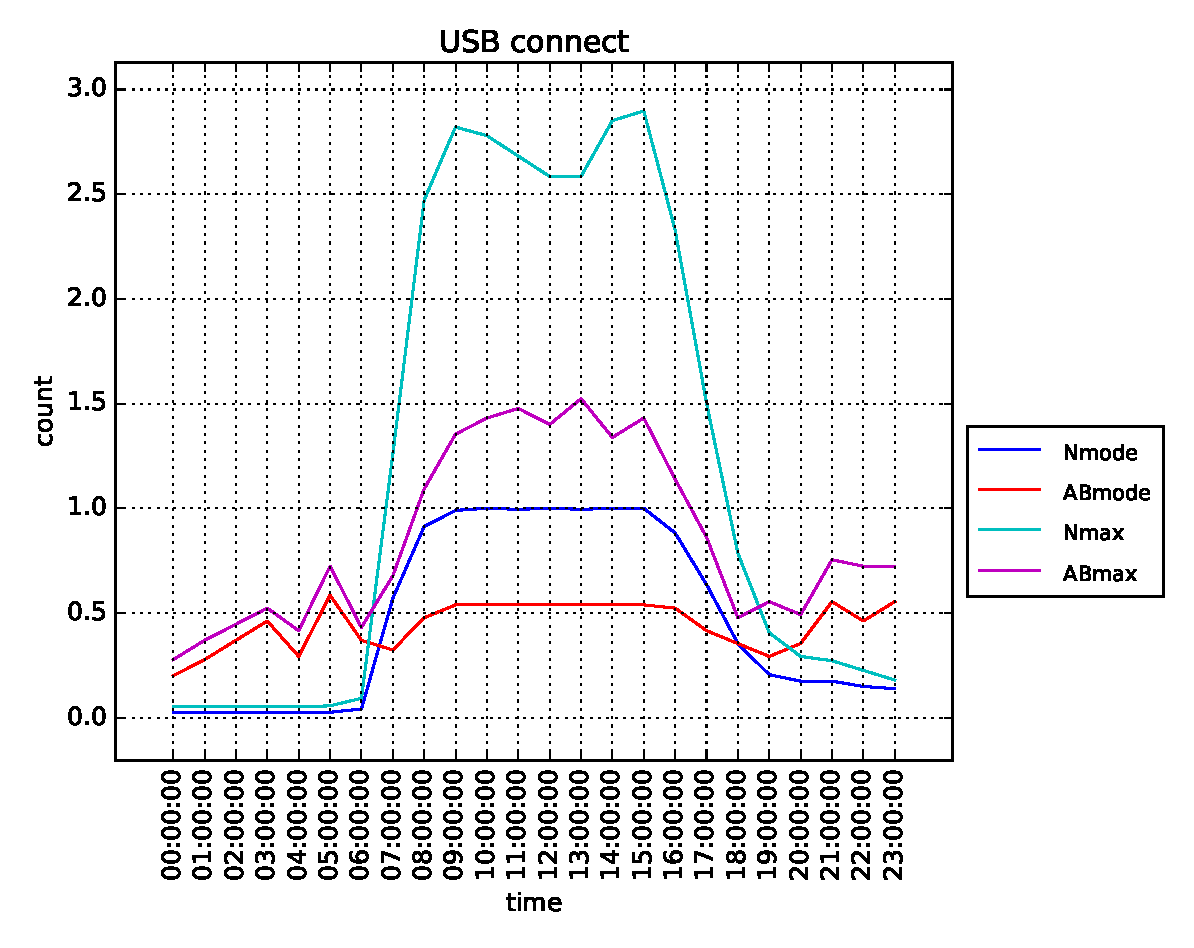
\includegraphics[width=0.18\textwidth]{figure/figure51.eps}
} 
\subfigure[USB disconnect]
{
 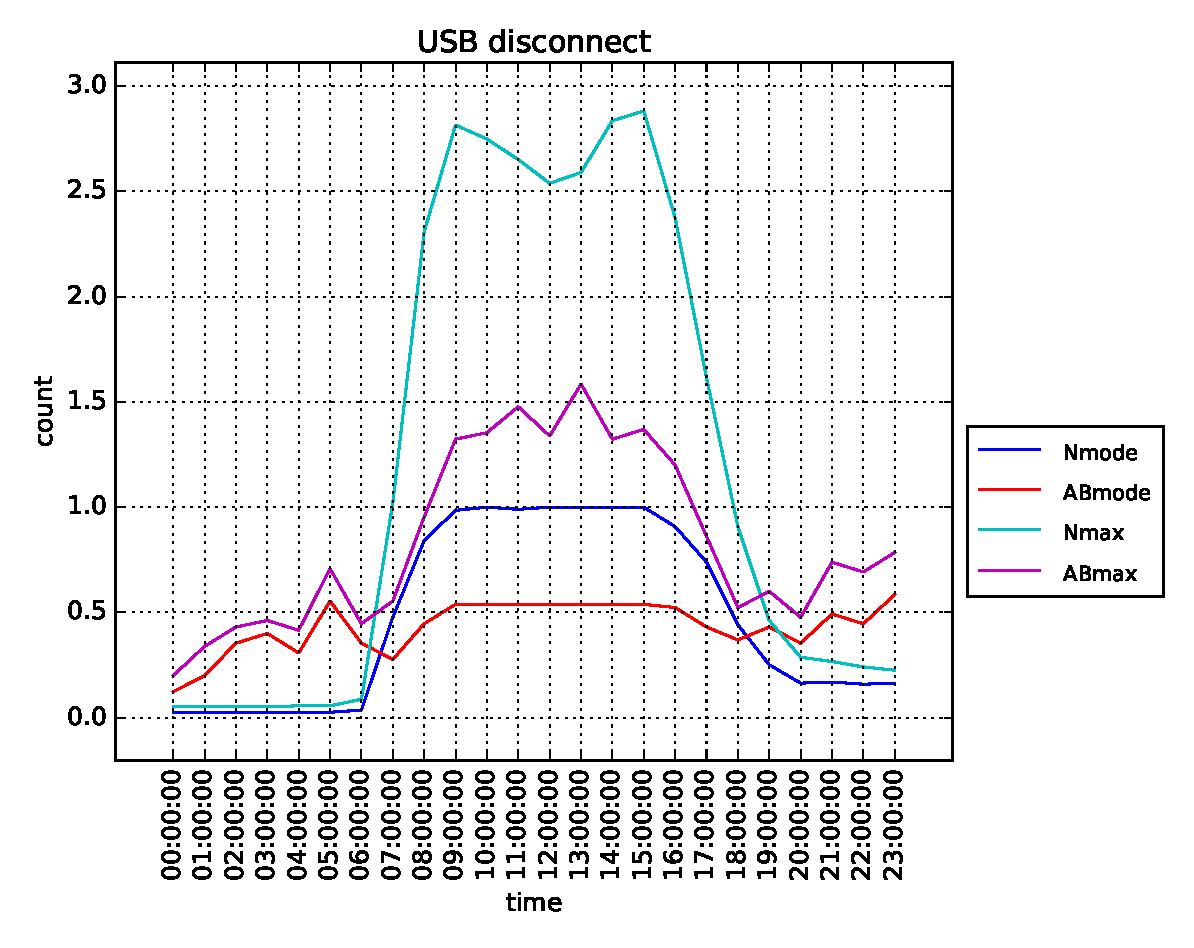
\includegraphics[width=0.18\textwidth]{figure/figure52.eps}
}
\subfigure[File copy]
{
 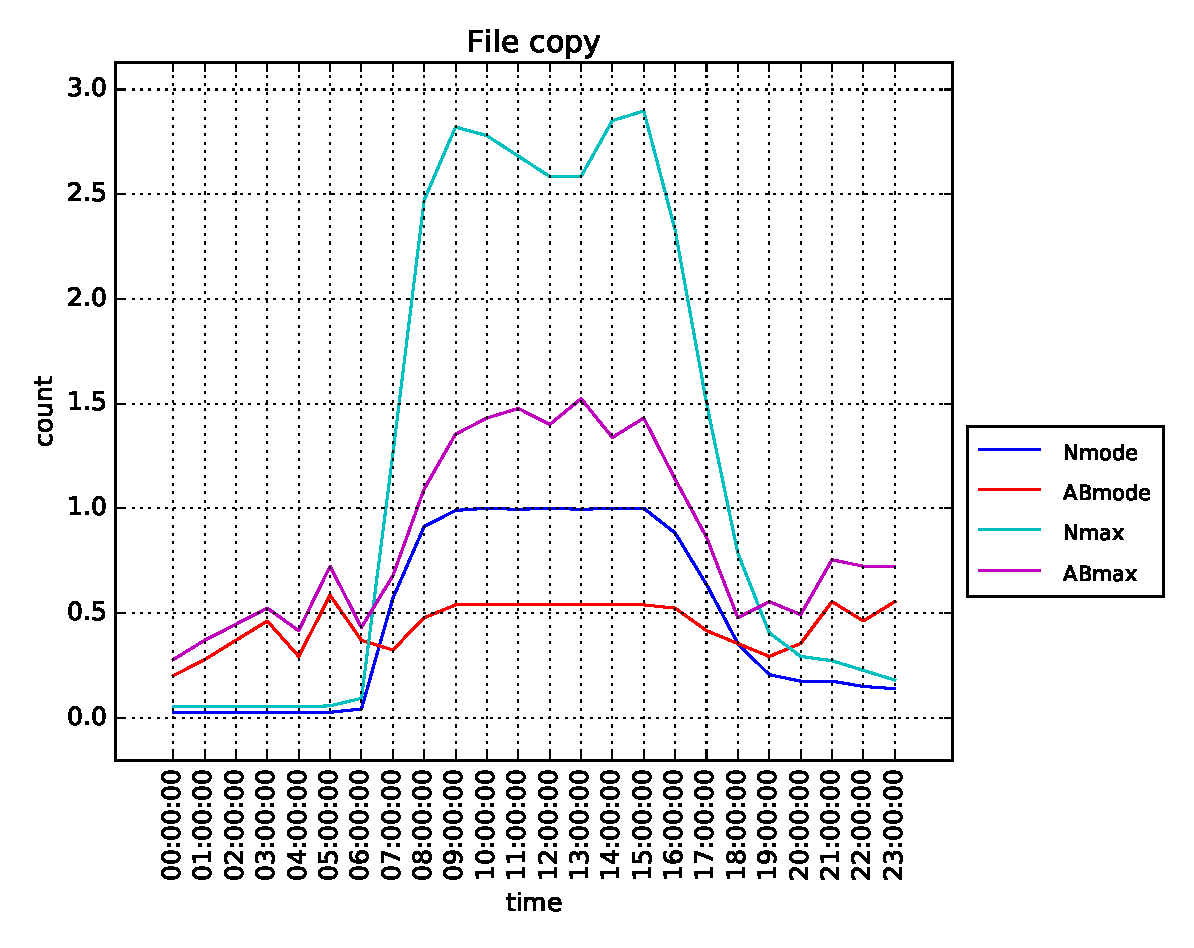
\includegraphics[width=0.18\textwidth]{figure/figure53.eps}
}
\caption{  Users' behaviors. 
``Nmode/Nmax'' presents the mode/max number of normal users behaviors, and
the ``ABmode/ABmax'' presents the mode/max number of abnormal users
behaviors. }
\label{fig4}
\end{figure*}

\noindent \textbf{Removable media usage.}
Removable media is among the most popular method used in theft of Intellectual Property  \cite{b18}. Tracking the use of removable media can be an excellent information source for identifying suspicious events.

\noindent \textbf{File copy Behaviors.}
File copying is an easy method to steal confidential evidence from organizations. So the number of occurrences of the behavior can give some useful information to detect insider threats. 

To model users' behaviors, we extract several temporal features to present the occurrences of different behaviors. For each user, we first count the times of each behavior for every hour, and then calculate the average of the maximum counts and mode counts of each behavior. The maximum counts indicate the change range of user behaviors, and the mode counts present the general behavior of most users. 
In order to find out whether the number of occurrences of these behaviors is different between normal users and abnormal users, figure 3 investigates their distributions.
\iffalse
we let the ``Nmode'' presents the mode number of normal users behaviors, and the ``ABmode'' presents the mode number of abnormal users behaviors. The maximum is the same with mode number.

Figure 3 is an indication of the distribution of users behaviors counts. 
\fi
We found that there is a big difference in behavior between normal users and abnormal users at different times in a day. Compared with normal users, these abnormal users have more frequent operations in midnight. So, we divide the 24 hours of a day into 4 time segments: (0:00-06:00),(00:60-12:00),(12:00-18:00),(18:00-24:00). The maximum or mode counts of user behaviors with regard to the five domains are calculated for the 4 segments respectively. Table 1 is an illustration of the feature set.

\begin{table}[tbp]
\caption{Selected feature set.}
\centering  % 表居中
\begin{tabular}{lll}  % {lccc} 表示各列元素对齐方式,left-l,right-r,center-c
\hline
Module    &\tabincell{c}{Features\\
(per 6 hours)} &\tabincell{c}{The number\\
of features}\\ \hline
    
Logon events    &Max/Mode Logon counts per 6 hours& 4\\\hline

Logoff events    &Max/Mode Logoff counts per 6 hours& 4\\\hline

Removable Media    &\tabincell{c}{Max/Mode USB connect  counts per 6 hours\\Max/Mode USB disconnect counts per 6 hours} &\tabincell{c}{4 \\ 4}\\\hline

File copy events    & Max/Mode Filecopy counts per 6 hours& 4\\\hline

\end{tabular}

\end{table}

\iffalse
In addition, in order to discover features which interfere with the ability to
correctly identify insider threats, we use PCA \cite{b19} for denoising.
\fi
In addition, in order to select domain features that have big impacts on user's behavior, we apply the Principal Component Analysis (PCA) \cite{b19} to give a score value to each feature. These features that obtain high scores are used to be the input to the model. 
\subsubsection{Anomaly Detection}

Due to the complex nature of insider threat problem, it is extremely hard to pinpoint a user as a malicious insider. This section focuses on implementing an anomaly detection algorithm based on the properties identified in the section of feature extraction. The anomaly detection algorithm adopted in this analysis is the ``Isolation forest (iforest)'' algorithm \cite{b20}, which stands out in effectively separating anomalous events from the rest of the instances. In the end, the iforest gives an anomaly score \emph{$R_{ADAD}$} for each user and outputs some users who may be an insider threat explicitly.

\subsection{Approach 2: Across-Time Anomaly Detection (ATAD)}

In this section, an improved model (IM) based on Markov is proposed to detect insider threats. We first build a model to represent the regular behaviors of a user. Then, we compare the temporal behavior in the recent past with the regular behaviors to detect unusual changes of his/her behaviors.
 
\iffalse
Figure 6 shows a graphical overview of the processing approach and pipeline we use, and the remainder of this section is dedicated to describing each stage in it.
\begin{figure}[htb]
\centerline{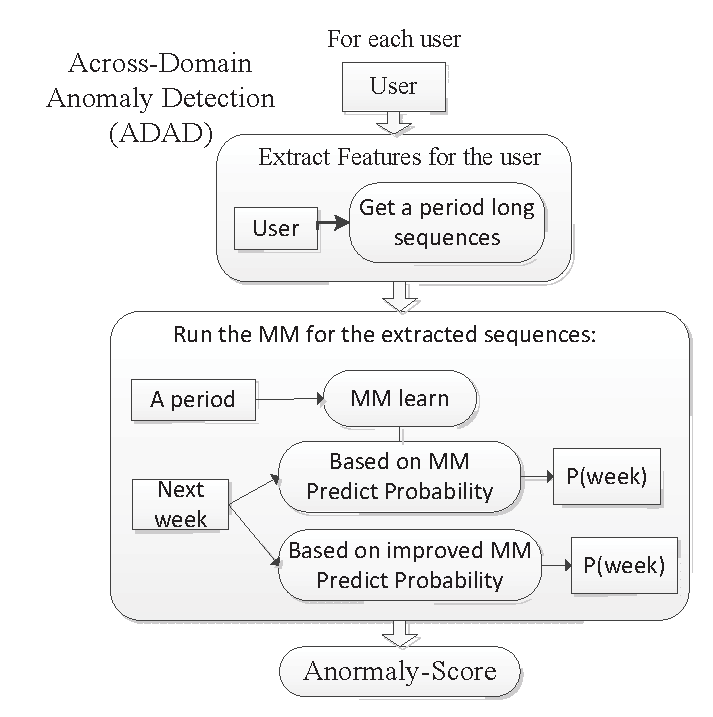
\includegraphics[width = 0.35\textwidth]{figure/figure6.eps}}
\caption{An overview of the Across-Time Anomaly Detection (ATAD).}
\label{fig}
\end{figure}
\fi
\subsubsection{Model building}

When building an improved model (IM), we take users behaviors as a temporal sequence and model users behaviors as Markov model (MM).
MM \cite{b21} is an extremely powerful
tool to model temporal sequence information. It has been
widely used in temporal pattern recognition problems (e.g.,
speech recognition, bioinformatics, gesture recognition) \cite{b23}. MM has also been used
in the area of intrusion detection \cite{b21}.

Users have different behaviors on computers every day. 
The historical behaviors of a user can be represented as a sequence of observations \emph{B=$(a_1,a_2...,a_n)$}, in which \emph{$a_i$} is the behavior that user is served by at time \emph{i}. 

Let substring \emph{B$(i, j) = a_ia_{i+1}\ldots a_j$} for any \emph{$1 \leq i \leq j \leq n$}. Define the context \emph{$c = B(n,n)$}. Let \emph{A} be the set of all possible behaviors. Also, we denote the user's behaviors as a random variable \emph{X}. 
For all \emph{$a \in A $} and \emph{$i \in \{1,2,. . ., n\}$}, the notation \emph{$P(X_i = a_i|\ldots)$} denotes the probability that \emph{$X_i$} takes the value \emph{$a_i$}.
These probabilities that can be represented by a \emph{transition
probability matrix M}. 
In order to obtain \emph{M}, we generate an estimate \emph{$\hat P$} from the current history \emph{B} using the current context \emph{c}. The probability for the next transition symbol to be \emph{a} is
\begin{align}
    P(a)=\hat P(X_{n+1}=a|B)= \frac {N(ca,B)}{N(c,B)},
\end{align}
where \emph{N(s',s)} denotes the number of times the substring \emph{s'} occurs in the string \emph{s}.
\iffalse
The estimate predicts the symbol \emph{$a \in A$} with the maximum probability \emph{$\hat P(X_{n+1}=a|B)$}; that is, the symbol that most frequently followed the current context \emph{c} in prior occurrences in the history. We will introduce the anomaly detection based on MM in the next section.
\fi

\subsubsection{Anomaly Detection}


We define the temporal behaviors in the recent past by opening up \emph{D} continuous observation windows with the length of \emph{N}. The users behaviors in the \emph{i-th} observation window is defined  \emph{$B_i$}=\emph{$a_{i1},a_{i2},\dots,a_{iN}$}, where \emph{N} denotes the \emph{N-th} behavior in the window \emph{i}.
Given the \emph{M} matrix produced in the first step, the anomaly score \emph{R$_{ATAD}$} for the user is calculated as
\begin{align}
R_{ATAD}=\frac{\sum_{d=1}^D \prod_{n=1}^N P(a_{dn})}{D},
\end{align}


After obtaining the anomaly score for all users, 
we set a threshold \emph{T}, which is used to classify users as anomalous or not. If the anomaly score of the user is below the threshold, he/she is identified as anomalous. This threshold \emph{T} is a critical parameter of our model which must be set carefully.
However, after running the IM algorithm, we can save the anomaly scores generated and then experiment with many values of \emph{T}. One could also imagine a human security analyst increasing T from 0 in order to be presented with more instances which the user deems anomalous.
\subsection{Information fusion}
In this section, our goal is to combine anomaly scores that have been generated from the two models proposed above and achieves a higher detection accuracy.
Therefore, a technique based on weight fusion is developed to combine the anomaly sores derived  from ADAD and ATAD. The combined anomaly score \emph{$R_{combine}$} is computed as
\iffalse
\begin{align}
R_{combine}&= W_1*R_{ADAD}+W_2*R_{ATAD}\\
r&=\begin{cases}
\frac{W_2}{W_1}
&\mbox{if } W_1 \textgreater 0\\
1
&\mbox{if } W_1 = 0,\\
\end{cases}
\end{align}
\fi
\begin{align}
R_{combine}&= W*R_{ATAD}+(1-W)*R_{ADAD}
\end{align}

where \emph{$R_{ADAD}$}/\emph{$R_{ATAD}$} denotes the anomaly score of ADAD/ATAD, and \emph{W} denotes the weight of \emph{$R_{ATAD}$}.
We then set a threshold \emph{$T_{combine}$}, which is used to classify users as anomalous or not. If the anomaly score of the user is below the threshold, we regard the user as anomalous.

\section{Experiment}
\iffalse
This section is dedicated to a comprehensive discussion of the results of the experiment.
We will first introduce the performance metrics for evaluating the three detection models,  separately. Then, we provide a comparative assessment of our proposed models with other existing insider threat detection methods. 
\fi
This section will provide a comprehensive evaluation on our proposed models. First, we assess the performance of ADAD, and then discuss the results of the ATAD. Finally, we 
provide a comparative assessment of our proposed hybrid model by comparing with the ADAD and ATAD.
\subsection{Across-Domain Anomaly Detection (ADAD)}\label{AA}
In this section, we first introduce the performance metrics for evaluating the detection model. 
Then, the model using distinct features are evaluated.

\emph{1) Evaluation Metrics and Baselines:}
Because the iforest identifies the anomalies, we evaluate the performance of this model by using \emph{accuracy, precision} and \emph{recall}.  
\emph{Precision} is the
fraction of the data entries labeled malicious that are
truly malicious; \emph{recall} is the fraction of malicious entries that are
classified correctly; \emph{accuracy} is the fraction of all entries
that are classified correctly \cite{b22}.
\iffalse
\emph{Accuracy} represents the proportion of the number of users who are detected correctly in all users by the model. \emph{precision} represents the proportion of the number of insider threats are detected correctly in the insider threats who are detected by the model and \emph{Recall} represents the proportion of the number of insider threats are detected in all insider threats by the model.
\fi

\iffalse
\begin{align}
Accuracy&= (TP+TN)/(TP+FP+TN+FN)\\
Precision&=TP/(TP+FP)\\
Recall&=TP/(TP+FN)
\end{align}
Where \emph{TP} denotes the number of insider threaters are detected as insider threaters, \emph{TN} denotes the number of normal users are detected normal users, \emph{FP} denotes the number of insider threaters are detected normal users and \emph{FN} denotes normal users are detected insider threaters.
\fi

\emph{2) Comparative Evaluation:} Table II shows the results of our models ADAD with different parameters.
We found that USB connect and disconnect are the most detectable. While logon and file domains are weak in detecting insider threats. It appears that normal users and abnormal users show great variations in their behavior of device usages, but are more uniform in the logon and file behaviors. Except that, the mode counts are more effective than maximum counts. The result indicates that the mode represents a more significant difference between the normal and the abnormal. It is obvious that some features interfere with the ability to correctly identify insider threats. 
The model can achieve a higher detection accuracy via decomposing the features to a 2-D space by \emph{PCA}, which denoises the data at the meantime.


\begin{table}[tbp]
\caption{The experiment result of ADAD.}
\centering  % 表居中
\begin{tabular}{lcccc}  % {lccc} 表示各列元素对齐方式,left-l,right-r,center-c
\hline
Domian  &Features &Accuracy &Precision &Recall\\ \hline
    
Logon     & MAX &89\% &32\% &47\%\\
  & MODE &87\% &22\% &34\%\\\hline
Logoff     & MAX &88\% &23\% &34\%\\
   & MODE &85\% &14\% &21\%\\\hline
USB connet     & MAX &78\% &65\% &27\%\\
  & MODE &79\% &70\% &28\%\\\hline
USB disconnect     & MAX &80\% &73\% &30\%\\
  & MODE &79\% &69\% &28\%\\\hline
Filecopy     & MAX &80\% &60\% &28\%\\
  & MODE &77\% &44\% &20\%\\\hline
All domains     & MAX &82\% &68\% &34\%\\
  & MODE &79\% &52\% &31\%\\\hline
\tabincell{c}{All domains combined \\with PCA method }    &   &\textbf{87\%} &\textbf{79\%} &\textbf{35\%}\\\hline

\end{tabular}

\end{table}


\subsection{Across-Time Anomaly Detection (ATAD)}
In this section, we first introduce the performance metrics for
evaluating the detection model. We then provide a
comparative assessment of our proposed models with existing MM detection methods.

\emph{1) Evaluation Metrics and Baselines:}
For ATAD, the threshold \emph{T} is essential to classify users as anomalous or not. 
So the metrics Receiver Operating Characteristic curves (or \emph{ROC} curves) is applied to evaluate the models \cite{b17}.

\textbf{Comparison Methods.}
MM is an extremely powerful tool to model temporal sequence information. It also been used in the general area of intrusion detection by some notable works \cite{b21}.
The IM is compared with existing detection model Markov.

\iffalse
Markov \cite{b21}: when calculating the anomaly score, this model regards the behavior sequences of the week as the whole, then calculates the probability of the behavior sequences as the anomaly score.
\fi
%This study let \emph{N} equal a day, and \emph{D} equal to a week for building a complete profile for a user as a week cycle.说一下训练集和测试集,选最后两个月的数据进行试验,因为时间太长会导致用户的行为发生变化。53天作为训练集,7天作为测试集。一个星期表示工作的一个cycle

\emph{2) Comparative Evaluation:} 
\textbf{Comparison between IM and MM.}
60 days from the 16th month to the 17th month of dataset R4.2.tar.bz has been used for ATAD. Specifically, the first 53 days in the 60 days is treated as the training set to build regular behaviors model and the rest is the testing set. Choosing 53 days as the training set can avoid the user's regular behaviors changing, which has an effect on building the normal model. The testing set is composed of records of a week, as behaviors of a week can build a complete work cycle profile for a user. IM mode sets the length of the observation window \emph{N} as a day.
The results of the IM model and MM model are shown in Fig. 4. It's obvious that the IM model is more effective than MM. For MM, if a user has once unusual change during this week, the change will have an important influence on the detection result. However, this effect can be avoided by IM. When scoring the user's behavior, IM uses the week's average anomaly score to evaluate a user's behavior, and reduces the impact of accidental unusual change on detecting insider threats.
\iffalse
In other words, IM tends to detect abnormal changes in behavioral trends over a period of time.
\fi
Hence, it detects insider threats more robustly. 



\begin{figure}[htb]
\centerline{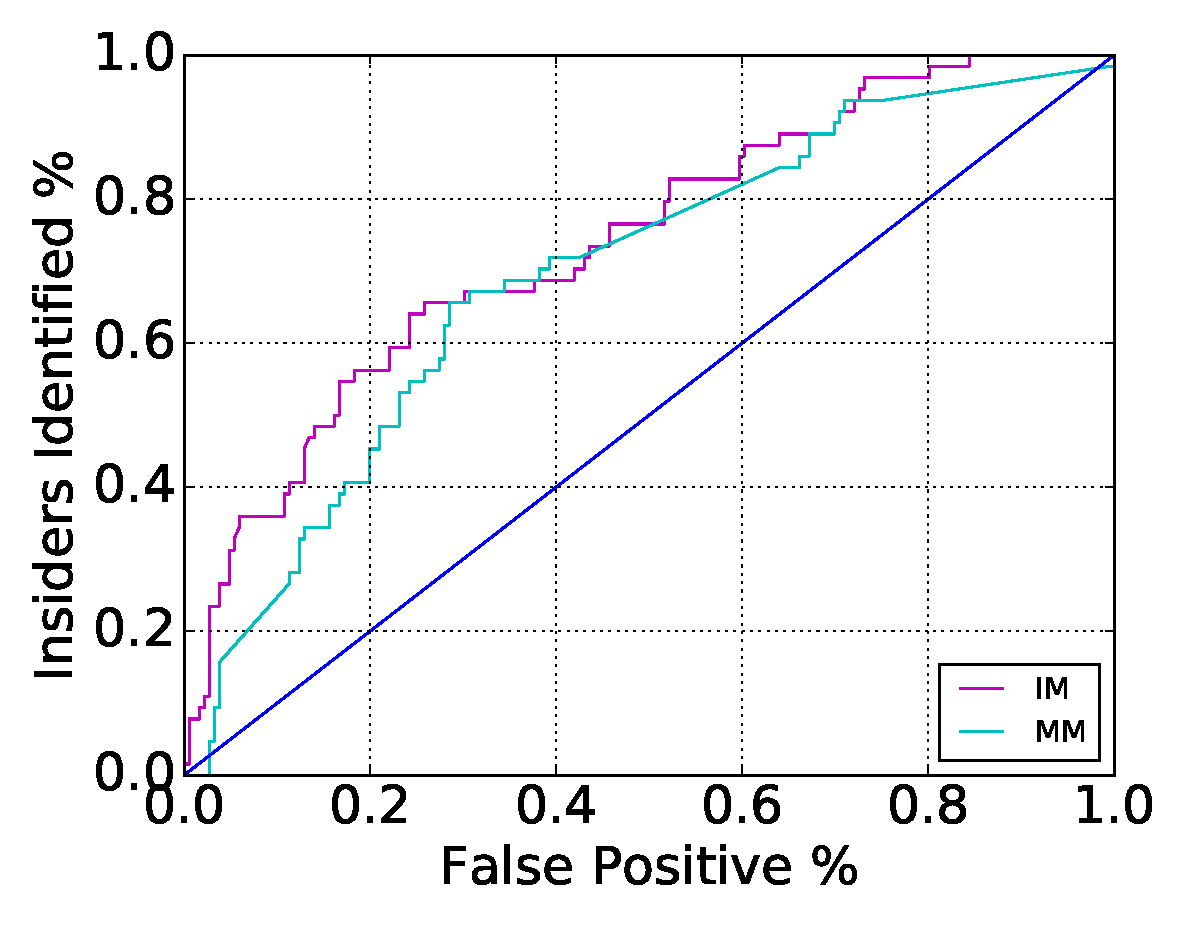
\includegraphics[width = 0.30\textwidth]{figure/figure7.eps}}
\caption{ROC Curve showing the differences between MM algorithm and IM algorithm.}
\label{fig}
\end{figure}


\subsection{Information fusion}
In this section,  we first introduce the performance metrics for evaluating the detection model.
We then provide a comparative assessment of our fusion method with the above two models.

\emph{1) Evaluation Metrics and Baselines:}
For the fusion method, the most important issue is to determine the weight of every component. So we let \emph{W}, the weight of ATAD, increase from 0 to 1. Then we use the metrics \emph{accuracy, precision} and \emph{recall} to quantitatively evaluate the models.

\emph{2) Comparative Evaluation:} 
We compare the fusion method with the ADAD and the ATAD, and the comparison results of detecting insider threats are shown in Table 3.
To remove amplitude variation and only focus on the underlying distribution shape on data, the scores are normalized before the weight fusion. When \emph{W} = 0, it is the result of individual ADAD method. When \emph{W} = 1, it is the result of individual ATAD method. We can see the ADAD is better than the ATAD, and fusing two model achieves better performance. When \emph{W} varies between 0.1 and 0.3, the precision of the hybrid model has greater improvements. The ADAD model is a data-driven model, and it fails to detect a malicious insider who tries to behave like a normal user to cover up his evil. However, the ATAD can make up for this deficiency by comparing behaviors of users in different time periods. So, it is remarkable to build a hybrid model to combine the individual ATAD and ADAD scores. 
\iffalse
\begin{table}[tbp]
\caption{The result of the information fusion experiment.}
\centering  % 表居中
\begin{tabular}{lcc}  % {lccc} 表示各列元素对齐方式,left-l,right-r,center-c
\hline
W  &Precision &Recall\\ \hline
0(ADAD) &79.17\% &35.19 \\\hline
0.1 &90\% &35.18\%\\\hline
0.2 &94.44\% &31.48\%\\\hline
0.3 &95\% &35.19\%\\\hline
0.4 &74.73\% &33.33\% \\\hline
0.5 &90\% &33.33\% \\\hline
0.6 &85\% &31.48\%\\\hline
0.7 &82.35\% &25.92\%\\\hline
0.8 &66.67\% &25.92\%\\\hline
0.9 &61.9\% &24.07\%\\\hline
1(ATAD) &60\% &27.78\%\\\hline
\end{tabular}

\end{table}
\fi


\begin{table*}[tbp]
\caption{The result of the information fusion experiment.}
\centering  % 表居中
\begin{tabular}{lccccccccccc}  % {lccc} 表示各列元素对齐方式,left-l,right-r,center-c
\hline
W &0(ADAD)&\textbf{0.1} &\textbf{0.2} &\textbf{0.3} &0.4 &0.5 &0.6 &0.7 &0.8 &0.9 &1(ATAD)\\\hline

Precision &79.17\% &\textbf{90\%} &\textbf{94.44\%} &\textbf{95\%}&74.73\%&90\%  &85\% &82.35\% &66.67\%&61.9\%&60\% \\\hline

Recall &35.19 &\textbf{35.18\%} &\textbf{31.48\%} &\textbf{35.19\%}&33.33\%&33.33\%&31.48\%&25.92\%&25.92\%&24.07\%&27.78\%\\\hline
\end{tabular}

\end{table*}

To get a better visualization of results based on our approach, we mark the positive sample with the red and negative sample with blue. 
When \emph{W} is 0.3, we chose a threshold 1.3 to determine insider threats.
Fig. 5 is an indication of how the anomaly scores are distributed when \emph{W} is 0.3. 
The purple color horizontal line is equivalent to the threshold.
Users whose anomaly scores exceed the threshold can be considered as anomalous users. The model exists some limitations. Our current procedure for determining if the
anomaly score is anomalous or not is to compare with a threshold. This requires us to manually set a threshold value, which is a hyperparameter of our mode that significantly affects the results. 
We will explore it in the future study. 
%indicates that 95\% of the insider threat we detected are true insider threats.  

\begin{figure}[htb]
\centerline{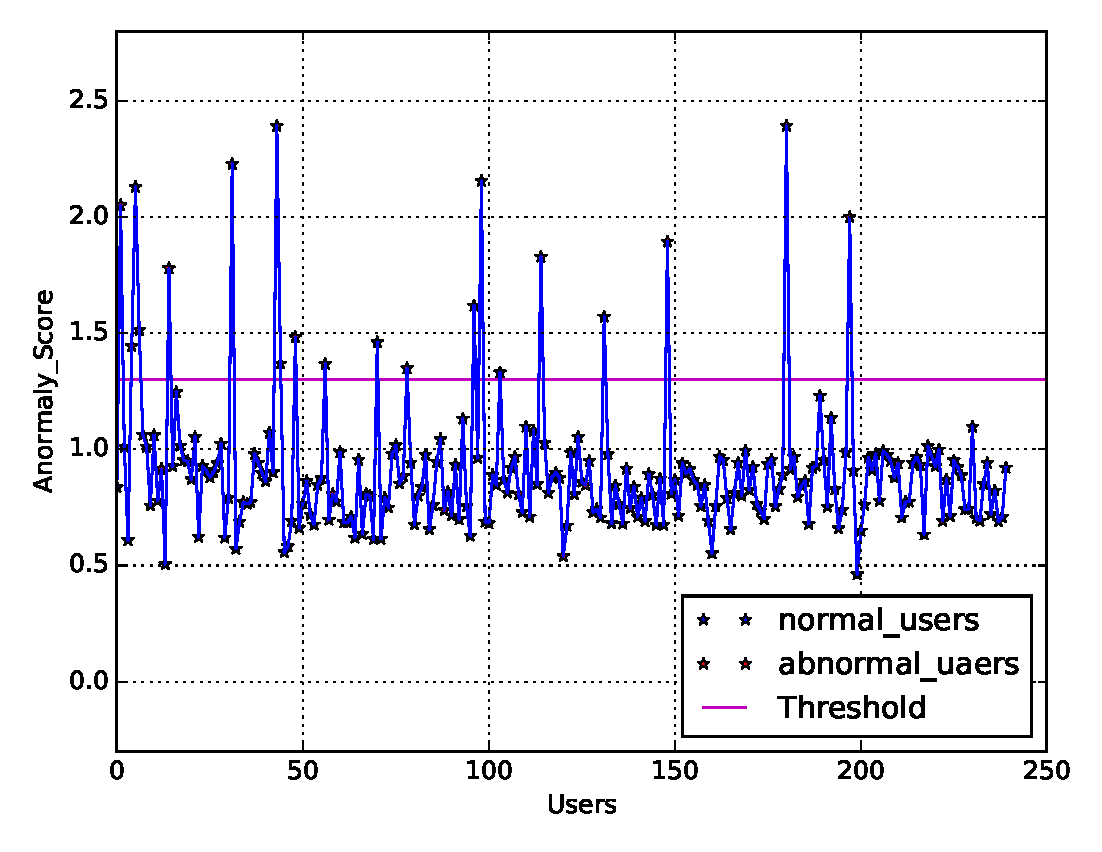
\includegraphics[width = 0.45\textwidth]{figure/figure8.eps}}
\caption{Anomaly score distribution.}
\label{fig}
\end{figure}

\section{Conclusion}

In this paper, we proposed a hybrid model that combined a data-driven model with a behavior-driven model to detect insider threat in a more robust and accurate manner. 
First, the multi-dimensional features extracted from data collected from the enterprise network is formatted and fed separately into the two separate models. Second, each model generated an abnormal score to represent the degree of users' unusual behaviors. Finally, the abnormal scores of two models were fused as the final abnormal scores for each user, and a user was detected as an insider threat if the anomaly score exceeded the threshold. After a wide range of experiments, it is verified that the hybrid model can detect insider threats with a high accuracy of 95\%, which is of great significance in industry and scientific research.

The proposed hybrid model has a high precision but a pessimistic recall. To solve this problem, we will take the user’s job role into account to improve the recall of anomaly detection  \cite{b16}.       



\section*{Acknowledgment}

This work was supported by the National Natural Science Foundation of China (No.61372062).



\begin{thebibliography}{00}
\bibitem{b1}Gavai, Gaurang, et al. "Detecting Insider Threat from Enterprise Social and Online Activity Data." ACM CCS International Workshop on Managing Insider Security Threats ACM, 2015:13-20.
\bibitem{b2} “By the numbers: Cyber attack costs compared,” 2016, accessed on 31/05/2016. [Online]. Available: http://www.csoonline.com/article/3074826/security/bythe-numbers-cyber-attack-costs-compared.html
\bibitem{b3}  D. Cappelli, A. Moore, and R. Trzeciak, The CERT Guide to Insider Threats: How to Prevent, Detect, and Respond to Information Technology Crimes (Theft, Sabotage, Fraud). Addison-Wesley Professional, 2012
\bibitem{b4} Young, William T, et al. Use of Domain Knowledge to Detect Insider Threats in Computer Activities.  2013.
\bibitem{b5} Rashid, Tabish, I. Agrafiotis, and J. R. C. Nurse. "A New Take on Detecting Insider Threats: Exploring the Use of Hidden Markov Models." International Workshop 2016:47-56.
\bibitem{b6}Eldardiry H, Sricharan K, Liu J, et al. Multi-source fusion for anomaly detection: using across-domain and across-time peer-group consistency checks[J]. Computing \& Informatics, 2014, 31(3):575-606.
\bibitem{b7}W. L. Winston, Operations Research: Applications and Algorithms. Belmont, CA: Duxbury Press, 1994.
\bibitem{b8} Sherali   Zeadally, et al. "Detecting Insider Threats: Solutions and Trends." Information Security Journal A Global Perspective 21.4(2012):183-192.
\bibitem{b9}  D. Cappelli, A. Moore, and R. Trzeciak, The CERT Guide to Insider Threats: How to Prevent, Detect, and Respond
to Information Technology Crimes (Theft, Sabotage, Fraud). Addison-Wesley Professional, 2012
\bibitem{b10} Gamachchi, Anagi, L. Sun, and S. Boztas. "A Graph Based Framework for Malicious Insider Threat Detection." Hawaii International Conference on System Sciences 2017.
\bibitem{b11}  P. A. Legg et al., “Towards a conceptual model and reasoning structure for insider threat detection,” J. Wireless Mobile Netw., Ubiquitous Comput., Dependable Appl., vol. 4, no. 4, pp. 20–37, Dec. 2013.
\bibitem{b12} M. Bishop et al., “Insider threat detection by process analysis,” in Proc. IEEE SPW, 2014, pp. 251–264.
\bibitem{b13} Sunu Mathew, Michalis Petropoulos, Hung Q Ngo, and Shambhu Upadhyaya. A data-centric approach to insider attack detection in database systems. In Recent Advances in Intrusion Detection, pages 382–401. Springer, 2010.
\bibitem{b14} William Eberle, Jeffrey Graves, and Lawrence Holder. Insider threat detection using a graph-based approach. Journal of Applied Security Research, 6(1):32–81, 2010.
\bibitem{b15} H. Eldardiry et al., “Multi-domain information fusion for insider threat detection,” in Proc. IEEE SPW, May 2013, pp. 45–51.
\bibitem{b16} Legg P A, Buckley O, Goldsmith M, et al. Automated Insider Threat Detection System Using User and Role-Based Profile Assessment[J]. IEEE Systems Journal, 2017, 11(2):503-512.
\bibitem{b17} Rashid, Tabish, I. Agrafiotis, and J. R. C. Nurse. "A New Take on Detecting Insider Threats: Exploring the Use of Hidden Markov Models." International Workshop 2016:47-56.
\bibitem{b18} D. Cappelli, A. Moore, and R. Trzeciak, The CERT Guide to Insider Threats: How to Prevent, Detect, and Respond
\bibitem{b19}I. Jolliffe, Principal Component Analysis. Hoboken, NJ, USA: Wiley,2005.
\bibitem{b20}F. T. Liu, K. M. Ting, and Z. H. Zhou, “Isolation forest,” in 2008 Eighth IEEE International Conference on Data Mining,
Dec 2008, pp. 413–422
\bibitem{b21} Ye, Nong. "A Markov Chain Model of Temporal Behavior for Anomaly Detection." 2000:171--174.
\bibitem{b22} Li, Ling Ko, et al. "Insider threat detection and its future directions." International Journal of Security \& Networks 12.3(2017):168.
\bibitem{b23} Lv, Qiujian, et al. "Big Data Driven Hidden Markov Model Based Individual Mobility Prediction at Points of Interest." IEEE Transactions on Vehicular Technology PP.99(2016):1-1.












\iffalse
\bibitem{b1}A. M. Dawn Cappelli Randall Trzeciak,Timothy J. Shimeall,“Common Sense Guide to Prevention and Detection of Insider
Threats , 3rd Edition,” 2009.
\bibitem{b2} Gemalto. Breach level index|data breach database \& risk assessment calculator, 2016. http://www.breachlevelindex.com/.
\bibitem{b3} “By the numbers: Cyber attack costs compared,” 2016, accessed on 31/05/2016. [Online]. Available: http://www.csoonline.com/article/3074826/security/bythe-numbers-cyber-attack-costs-compared.html
\bibitem{b4} Teresa F Lunt. A survey of intrusion detection techniques. Computers \& Security, 12(4):405–418, 1993.
\bibitem{b5} Sunu Mathew, Michalis Petropoulos, Hung Q Ngo, and Shambhu Upadhyaya. A data-centric approach to insider attack detection in database systems. In Recent Advances in Intrusion Detection, pages 382–401. Springer, 2010.
\bibitem{b6} William Eberle, Jeffrey Graves, and Lawrence Holder. Insider threat detection using a graph-based approach. Journal of Applied Security Research, 6(1):32–81, 2010.
\bibitem{b7} Alex Memory, Henry G Goldberg, and E Ted. Context-aware insider threat detection. In Workshops at the Twenty-Seventh AAAI Conference on Artificial
Intelligence, 2013.
\bibitem{b8} Robert F Mills, Michael R Grimaila, Gilbert L Peterson, and Jonathan W Butts. A scenario-based approach to mitigating the insider threat. Technical report, DTIC Document, 2011.
\bibitem{b9}  D. Cappelli, A. Moore, and R. Trzeciak, The CERT Guide to Insider Threats: How to Prevent, Detect, and Respond
to Information Technology Crimes (Theft, Sabotage, Fraud). Addison-Wesley Professional, 2012
\bibitem{b10}  Miltiadis Kandias, Alexios Mylonas, Nikos Virvilis, Marianthi Theoharidou, and Dimitris Gritzalis. An insider threat prediction model. In Trust, privacy and security in digital business, pages 26–37. Springer, 2010.
\bibitem{b11}Frank L Greitzer, Lars J Kangas, Christine F Noonan,and Angela C Dalton. Identifying at-risk employees: A behavioral model for predicting potential insider threats. Pacific Northwest National Laboratory Richland, WA, 2010
\bibitem{b12}GB Magklaras and SM Furnell. Insider threat prediction tool: Evaluating the probability of it misuse. Computers \& Security, 21(1):62–73, 2001.
\bibitem{b13}Hoda Eldardiry, Evgeniy Bart, Juan Liu, John Hanley, Bob Price, and Oliver Brdiczka. Multi-domain information fusion for insider threat detection. In Security and Privacy Workshops (SPW), 2013 IEEE, pages 45–51. IEEE, 2013.
\bibitem{b14}Automated Insider Threat Detection System Using User and Role-Based Profile Assessment Philip A. Legg, Oliver Buckley, Michael Goldsmith, and Sadie Creese
\bibitem{b15}  Deep Learning for Unsupervised Insider Threat Detection in Structured Cybersecurity Data Streams Aaron Tuor and Samuel Kaplan and Brian Hutchinson∗
Western Washington University Bellingham, WA Nicole Nichols and Sean Robinson Pacific Northwest National Laboratory Seattle, WA
\bibitem{b16}  P. A. Legg et al., “Towards a conceptual model and reasoning structure for insider threat detection,” J. Wireless Mobile Netw., Ubiquitous Comput., Dependable Appl., vol. 4, no. 4, pp. 20–37, Dec. 2013.
\bibitem{b17} M. Bishop et al., “Insider threat detection by process analysis,” in Proc. IEEE SPW, 2014, pp. 251–264.
\bibitem{b18}] M. Bishop, S. Engle, S. Peisert, S. Whalen, and C. Gates, “We have met the enemy and he is us,” in Proc. NSPW, Lake Tahoe, CA, USA, Sep. 2008, pp. 1–12
\bibitem{b19} J. R. C. Nurse et al., “Understanding insider threat: A framework for characterising attacks,” in Proc. IEEE SPW, 2014, pp. 214–228
\bibitem{b20}F. Kammueller and C. W. Probst, “Invalidating policies using structural information,” J. Wireless Mobile Netw., Ubiquitous Comput., Dependable Appl., vol. 5, no. 2, pp. 59–79, Jun. 2014.
\bibitem{b21} M. R. Ogiela and U. Ogiela, “Linguistic protocols for secure information management and sharing,” Comput. Math. Appl., vol. 63, no. 2, pp. 564–572, Jan. 2012.
\bibitem{b22}G. B. Magklaras and S. M. Furnell, “Insider threat prediction tool: Evaluating the probability of IT misuse,” Comput. Security, vol. 21, no. 1, pp. 62–73, 1st Quart. 2002.
\bibitem{b23} L. Spitzner, “Honeypots: Catching the insider threat,” in Proc. 19th IEEE ACSAC, Las Vegas, NV, USA, Dec. 2003, pp. 170–179.
\bibitem{b24}G. B. Magklaras and S. M. Furnell, “Insider threat prediction tool: Evaluating the probability of IT misuse,” Comput. Security, vol. 21, no. 1, pp. 62–73, 1st Quart. 2002.
\bibitem{b25} J. Myers, M. R. Grimaila, and R. F. Mills, “Towards insider threat detection using web server logs,” in Proc. 5th Annu. CSIIRW—Cyber Security Inf. Intell. Challenges Strategies, New York, NY, USA, 2009, pp. 54:1–54:4.
\bibitem{b26} M. A. Maloof and G. D. Stephens, “Elicit: A system for detecting insiders who violate need-to-know,” in Recent Advances in Intrusion Detection, vol. 4637, Lecture Notes in Computer Science, C. Kruegel, R. Lippmann, and A. Clark, Eds. Berlin, Germany: Springer-Verlag, 2007, pp. 146–166.
\bibitem{b27} J. S. Okolica, G. L. Peterson, and R. F. Mills, “Using PLSI-U to detect insider threats by datamining e-mail,” Int. J. Security Netw., vol. 3, no. 2, pp. 114–121, 2008.
\bibitem{b28}Y. Liu et al., “SIDD: A framework for detecting sensitive data exfiltration sby an insider attack,” in Proc. 42nd HICSS, Jan. 2009, pp. 1–10.
\bibitem{b29} H. Eldardiry et al., “Multi-domain information fusion for insider threat detection,” in Proc. IEEE SPW, May 2013, pp. 45–51.
\bibitem{b30} Brdiczka et al., “Proactive insider threat detection through graph learning and psychological context,” in Proc. IEEE Symp. SPW, San Francisco, CA, USA, May 2012, pp. 142–149.
\bibitem{b31}W. Eberle, J. Graves, and L. Holder, “Insider threat detection using a graph-based approach,” J. Appl. Security Res., vol. 6, no. 1, pp. 32–81, Dec. 2010.
\bibitem{b32}B. Klimt and Y. Yang, “The enron corpus: A new dataset for email classification research,” in Machine Learning: ECML 2004, vol. 3201, Lecture Notes in Computer Science, J.-F. Boulicaut, F. Esposito, F. Giannotti, and D. Pedreschi, Eds. Berlin, Germany: Springer-Verlag, 2004, pp. 217–226
\bibitem{b33}T. E. Senator et al., “Detecting insider threats in a real corporate database of computer usage activity,” in Proc. 19th ACM SIGKDD Int. Conf. Knowl. Discov. Data Mining, 2013, pp. 1393–1401.
\bibitem{b34}P. Parveen, J. Evans, B. Thuraisingham, K. W. Hamlen, and L. Khan, “Insider threat detection using stream mining and graph mining,” in Proc. IEEE 3rd Int. Conf. Social Comput. PASSAT, Oct. 2011, pp. 1102–1110.
\bibitem{b35}P. Parveen and B. Thuraisingham, “Unsupervised incremental sequence learning for insider threat detection,” in Proc. IEEE Int. Conf. ISI, Jun. 2012, pp. 141–143.
\bibitem{b36}S. Greenberg, Using unix: Collected traces of 168 users, Univ. Calgary, Calgary, AB, Canada, Tech. Rep., 1988.
\bibitem{b37} Rashid, Tabish, I. Agrafiotis, and J. R. C. Nurse. "A New Take on Detecting Insider Threats: Exploring the Use of Hidden Markov Models." International Workshop 2016:47-56.
\bibitem{b38}Automated Insider Threat Detection System Using User and Role-Based Profile Assessment Philip A. Legg, Oliver Buckley, Michael Goldsmith, and Sadie Creese
\bibitem{b39}“CERT Insider Threat Data Set,” Software Engineering Institute, Carnegie Mellon University, CERT Division and Exact
Data LLC. [Online]. Available: https://www.cert.org/insiderthreat/tools/
\bibitem{b40}D. Cappelli, A. Moore, and R. Trzeciak, The CERT Guide to Insider Threats: How to Prevent, Detect, and Respond
to Information Technology Crimes (Theft, Sabotage, Fraud). Addison-Wesley Professional, 2012.
\bibitem{b41} D. Cappelli, A. Moore, and R. Trzeciak, The CERT Guide to Insider Threats: How to Prevent, Detect, and Respond
to Information Technology Crimes (Theft, Sabotage, Fraud). Addison-Wesley Professional, 2012.
\bibitem{b42}I. Jolliffe, Principal Component Analysis. Hoboken, NJ, USA: Wiley,2005.
\bibitem{b43}F. T. Liu, K. M. Ting, and Z. H. Zhou, “Isolation forest,” in 2008 Eighth IEEE International Conference on Data Mining,
Dec 2008, pp. 413–422
\bibitem{b44}L. Sun, S. Versteeg, S. Boztas, and A. Rao, “Detecting anomalous user behaviour using an extended Isolation Forest algorithm: An enterprise case study,” Sept 2016, arXiv:1609.06676.
\bibitem{b45}W. L. Winston, Operations Research: Applications and Algorithms. Belmont, CA: Duxbury Press, 1994.
\bibitem{b46}W. L. Winston, Operations Research: Applications and Algorithms. Belmont, CA: Duxbury Press, 1994.
\bibitem{b47}T. M. Mitchell, Machine Learning. Boston,
MA: McGraw-Hill, 1997.
\bibitem{b48} J. R. C. Nurse, O. Buckley, P. A. Legg, M. Goldsmith, S. Creese, G. R. Wright, and M. Whitty. Understanding insider threat: A framework for characterising attacks. In IEEE Security and Privacy Workshops (SPW). IEEE, 2014. DOI: 10.1109/SPW.2014.38.
\bibitem{b49}Eldardiry H, Sricharan K, Liu J, et al. Multi-source fusion for anomaly detection: using across-domain and across-time peer-group consistency checks[J]. Computing \& Informatics, 2014, 31(3):575-606.
\bibitem{b50} Legg P A, Buckley O, Goldsmith M, et al. Automated Insider Threat Detection System Using User and Role-Based Profile Assessment[J]. IEEE Systems Journal, 2017, 11(2):503-512.
\bibitem{b51} Young, William T, et al. Use of Domain Knowledge to Detect Insider Threats in Computer Activities.  2013.
\bibitem{b52} Gamachchi, Anagi, L. Sun, and S. Boztas. "A Graph Based Framework for Malicious Insider Threat Detection." Hawaii International Conference on System Sciences 2017.

\bibitem{b53} Sherali   Zeadally, et al. "Detecting Insider Threats: Solutions and Trends." Information Security Journal A Global Perspective 21.4(2012):183-192.

\bibitem{b54} Ye, Nong. "A Markov Chain Model of Temporal Behavior for Anomaly Detection." 2000:171--174.
\bibitem{b55} Lv, Qiujian, et al. "Big Data Driven Hidden Markov Model Based Individual Mobility Prediction at Points of Interest." IEEE Transactions on Vehicular Technology PP.99(2016):1-1.

\bibitem{b56} Li, Ling Ko, et al. "Insider threat detection and its future directions." International Journal of Security & Networks 12.3(2017):168.

\fi








\end{thebibliography}

\end{document}
